\documentclass[10pt]{beamer}

%%%
% PREAMBLE FOR THIS DOC 
%%%
%https://tex.stackexchange.com/questions/68821/is-it-possible-to-create-a-latex-preamble-header
\usepackage{/Users/miw267/Repos/csci246_spring2025/slides/preambles/beamer_preamble_for_CSCI246}



%%% TRY TO RESHOW TOC AT EACH SECTION START (with current section highlighted)
% Reference: https://tex.stackexchange.com/questions/280436/how-to-highlight-a-specific-section-in-beamer-toc
\newcommand\tocforsect[2]{%
  \begingroup
  \edef\safesection{\thesection}
  \setcounter{section}{#1}
  \tableofcontents[#2,currentsection]
  \setcounter{section}{\safesection}
  \endgroup
}



%%%% HERES HOW TO DO IT CORRECTLY
% FIRST IN .STY FILE, DO
%\usetheme[sectionpage=none]{metropolis}
% THEN AT EACH SECTION DO
%\begin{frame}{Outline}
%  \tableofcontents[currentsection]	
%\end{frame}



%\setbeamertemplate{navigation symbols}{}
%\setbeamertemplate{footline}[frame number]{}


%%%
% DOCUMENT
%%%

\begin{document}

%\maketitle

%% Title page frame
%\begin{frame}
%    \titlepage 
%\end{frame}





\title{02/21/2025: Introduction to Functions}
\author{CSCI 246: Discrete Structures}
\date{Textbook reference: Ch 11.5, Hampkins}

\begin{frame}
    \titlepage 
\end{frame}


\begin{frame}
\footnotesize 
\begin{mygreenbox}[title=Graded Quiz Pickup]
Quizzes are in the front of the room, grouped into four bins (A-G, H-L, M-R, S-Z) by last name. The quizzes are upside down with your last name on the back. Come find yours before, during, or after class.  Only turn the quiz over if it's yours.
\end{mygreenbox} 
\vfill 

\begin{myredbox}[title=Announcements]

\begin{itemize}
\item I have not yet completed requested regrades that were handed to me last class. 
\end{itemize}

\end{myredbox}

\vfill 


\begin{myyellowbox}[title=Today's Agenda]
\begin{itemize}
	\item Reading + problems quizzes (15 mins)
	\item Mini-lecture ($\approx$ 15 mins)
%	%
%	\begin{itemize}
%	\footnotesize 
%	\item Review induction 
%	\end{itemize}
%	%
	\item Group exercises ($\approx$ 15 mins)
\end{itemize}

\end{myyellowbox}
\vfill 

\end{frame}




\begin{frame}
\footnotesize 

 \begin{myredbox}[title=Reading Quiz (Extra Credit)]     \centering
State whether each relationship below is a function or not.  If it is a function, state whether the function is injective (1-to-1), surjective (onto), both, or neither.
    \scalebox{0.9}{\begin{tabular}{ccccc}
    (a) & (b) & (c) & (d) & (e) \\
   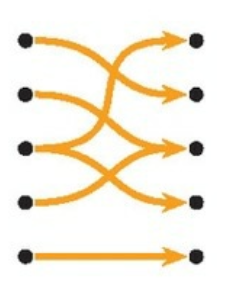
\includegraphics[width=0.18\textwidth]{images/function5}  &
    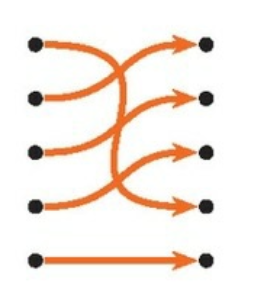
\includegraphics[width=0.18\textwidth]{images/function4}  & 
    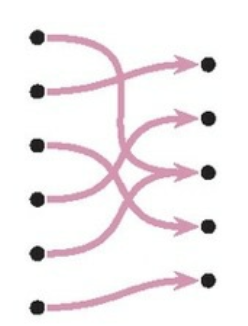
\includegraphics[width=0.18\textwidth]{images/function3}  & 
    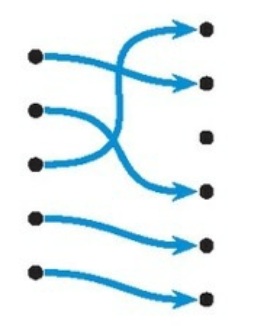
\includegraphics[width=0.18\textwidth]{images/function2}  & 
    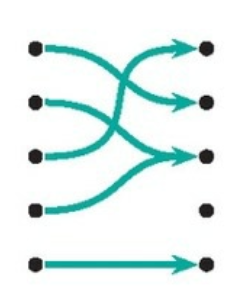
\includegraphics[width=0.18\textwidth]{images/function1} \\   
    \end{tabular}}
\end{myredbox}


 \vfill

 \begin{mygreenbox}[title=Problems Quiz (Quantifiers and Set Operations)]
\begin{enumerate}
	\item  
 Label each sentence below about the integers as true or false. 
 \vspace{-0.15cm}
	\begin{columns}
	    \column{0.50\textwidth}  % First column (50% of slide width)
	    \begin{align*}
	       \text{(a)} &\; \exists x, \exists y: x+y=0. \\
	        \text{(b)} & \; \forall x, \forall y, x+y=0. \\ 
	      \text{(c)} & \; \exists x: \forall y, x+y=0. \\ 
	         \text{(d)} & \; \forall x, \exists y: x+y=0           
	      \end{align*}
	
	    \column{0.50\textwidth}  % Second column (50% of slide width)
	    \begin{align*} 
	       \text{(e)} &\; \exists x, \exists y: xy=0. \\
	        \text{(f)} & \; \forall x, \forall y, xy=0.  \\
	      \text{(g)} & \; \forall x, \exists y: xy=0. \\
	        \text{(h)} & \; \exists x: \forall y, xy=0. 
	    \end{align*}
	\vfill 
	\end{columns}
   \item How many integers in the range 1 to 1000 (inclusive) are divisible by 2 or by 5?  Justify your answer. \textbf{Hint:} If $A$ and $B$ be finite sets.  Then \quad $|A| + |B| = |A \cup B| + |A \cap B|$.
\end{enumerate}
\end{mygreenbox}



\end{frame}


\begin{frame}[standout]
Additional notes on relations
\end{frame}



\begin{frame}
\footnotesize 
\begin{myredbox}[title=Reminder of Definition]
Given sets $A$ and $B$ the \textbf{Cartesian Product} $A \times B$ is just the set of ordered pairs $(a,b)$ where $a \in A, b \in B$.
\end{myredbox}

\vfill 
\begin{mygreenbox}[title=Example]
Suppose $A=\set{1,2,3,4}$ and $B=\set{1,2,3,4,5}$.  Then the set $A \times B$ is given by 


    \[
    \begin{array}{ccccccc}
        \bigg\{ & (1,1), & (1,2), & (1,3), & (1,4), & (1,5),& \\
        & (2,1), & (2,2), & (2,3), & (2,4), & (2,5), &\\
        &(3,1), & (3,2), & (3,3), & (3,4), & (3,5), &\\
        &(4,1), & (4,2), & (4,3), & (4,4), & (4,5) & \bigg\} \\
    \end{array}
    \]
\end{mygreenbox}

\vfill 
\begin{mygreenbox}[title=Example]
Suppose $A=\set{a,b,c}$ and $B=\set{a,b,c,d,e,f}$.  Then the set $A \times B$ is given by 
   \[
    \begin{array}{cccccccc}
         \bigg\{ &  (a,a), & (a,b), & (a,c), & (a,d), & (a,e), & (a,f), & \\
        & (b,a), & (b,b), & (b,c), & (b,d), & (b,e), & (b,f), & \\
        & (c,a), & (c,b), & (c,c), & (c,d), & (c,e), & (c,f) & \bigg\} \\

    \end{array}
    \]
 \end{mygreenbox}
\end{frame}




\begin{frame}


\begin{myyellowbox}[title=Perspective on Relations]
Any \textit{relation} can be considered as a subset of $A \times B$.
\end{myyellowbox}

\begin{mygreenbox}[title=Example]
Suppose $A=B=\set{1,2,3,4,5}$.  Then the relation $\boxed{"\leq"}$ (more formally $\set{(a,b): a \leq b}$) includes (is satisfied by) the elements below shaded in green.
\vfill 

    \[
    \begin{array}{ccccccc}
        \bigg\{ &   \cellcolor{green!50} (1,1), & \cellcolor{green!50} (1,2), & \cellcolor{green!50} (1,3), & \cellcolor{green!50} (1,4), & \cellcolor{green!50} (1,5), &\\
         & \cellcolor{red!40} (2,1), & \cellcolor{green!50} (2,2), & \cellcolor{green!50} (2,3), & \cellcolor{green!50} (2,4), & \cellcolor{green!50} (2,5), &\\
        & \cellcolor{red!40} (3,1), & \cellcolor{red!40} (3,2), & \cellcolor{green!50} (3,3), & \cellcolor{green!50} (3,4), & \cellcolor{green!50} (3,5), &\\
        & \cellcolor{red!40} (4,1), & \cellcolor{red!40} (4,2), & \cellcolor{red!40} (4,3), & \cellcolor{green!50} (4,4), & \cellcolor{green!50} (4,5), & \\
        & \cellcolor{red!40} (5,1), & \cellcolor{red!40} (5,2), & \cellcolor{red!40} (5,3), & \cellcolor{red!40} (5,4), & \cellcolor{green!50} (5,5) & \bigg\} \\
    \end{array}
    \]
\end{mygreenbox}
\end{frame}


\begin{frame}


\begin{myyellowbox}[title=Perspective on Relations]
Any \textit{relation} can be considered as a subset of $A \times B$.
\end{myyellowbox}

\begin{mygreenbox}[title=Example]
Suppose $A=B=\set{1,2,3,4,5}$.  Then the relation $\boxed{"\geq"}$ (more formally $\set{(a,b): a \geq b}$) includes (is satisfied by) the elements below shaded in green.
\vfill 

   \[
    \begin{array}{ccccccc}
        \bigg\{ &   \cellcolor{green!50} (1,1), & \cellcolor{red!40} (1,2), & \cellcolor{red!40} (1,3), & \cellcolor{red!40} (1,4), & \cellcolor{red!40} (1,5), &\\
         & \cellcolor{green!50} (2,1), & \cellcolor{green!50} (2,2), & \cellcolor{red!40} (2,3), & \cellcolor{red!40} (2,4), & \cellcolor{red!40} (2,5), &\\
        & \cellcolor{green!50} (3,1), & \cellcolor{green!50} (3,2), & \cellcolor{green!50} (3,3), & \cellcolor{red!40} (3,4), & \cellcolor{red!40} (3,5), &\\
        & \cellcolor{green!50} (4,1), & \cellcolor{green!50} (4,2), & \cellcolor{green!50} (4,3), & \cellcolor{green!50} (4,4), & \cellcolor{red!40} (4,5), & \\
        & \cellcolor{green!50} (5,1), & \cellcolor{green!50} (5,2), & \cellcolor{green!50} (5,3), & \cellcolor{green!50} (5,4), & \cellcolor{green!50} (5,5) & \bigg\} \\
    \end{array}
    \]
\end{mygreenbox}
\end{frame}


\begin{frame}

\begin{myredbox}[title=Remark]
Whenever $A$ and $B$ are finite sets, we can draw (or imagine) a matrix of all possible ordered pairs $(a,b)$, and think about a relation in terms of properties of this matrix.
\end{myredbox}


\begin{mygreenbox}[title=Example]
If a relationship is \textbf{reflexive}, it must include all diagonal elements.

   \[
    \begin{array}{ccccccc}
        \bigg\{ &   \cellcolor{green!50} (1,1), & \cellcolor{yellow!50} (1,2), & \cellcolor{yellow!50} (1,3), & \cellcolor{yellow!50} (1,4), & \cellcolor{yellow!50} (1,5), &\\
         & \cellcolor{yellow!50} (2,1), & \cellcolor{green!50} (2,2), & \cellcolor{yellow!50} (2,3), & \cellcolor{yellow!50} (2,4), & \cellcolor{yellow!50} (2,5), &\\
        & \cellcolor{yellow!50} (3,1), & \cellcolor{yellow!50} (3,2), & \cellcolor{green!50} (3,3), & \cellcolor{yellow!50} (3,4), & \cellcolor{yellow!50} (3,5), &\\
        & \cellcolor{yellow!50} (4,1), & \cellcolor{yellow!50} (4,2), & \cellcolor{yellow!50} (4,3), & \cellcolor{green!50} (4,4), & \cellcolor{yellow!50} (4,5), & \\
        & \cellcolor{yellow!50} (5,1), & \cellcolor{yellow!50} (5,2), & \cellcolor{yellow!50} (5,3), & \cellcolor{yellow!50} (5,4), & \cellcolor{green!50} (5,5) & \bigg\} \\
    \end{array}
    \]
The yellow cells could be either included or excluded.
\end{mygreenbox}

\end{frame}


\begin{frame}
\begin{myredbox}[title=Remark]
Whenever $A$ and $B$ are finite sets, we can draw (or imagine) a matrix of all possible ordered pairs $(a,b)$, and think about a relation in terms of properties of this matrix.
\end{myredbox}


\begin{mygreenbox}[title=Example]
If a relationship is \textbf{symmetric}, then if some element is included, its transposed element must be included.  For example, 

    \[
    \begin{array}{ccccccc}
        \bigg\{ &   \cellcolor{red!40} (1,1), & \cellcolor{green!50} (1,2), & \cellcolor{red!40} (1,3), & \cellcolor{red!40} (1,4), & \cellcolor{red!40} (1,5), &\\
         & \cellcolor{green!50} (2,1), & \cellcolor{red!40} (2,2), & \cellcolor{red!40} (2,3), & \cellcolor{green!50} (2,4), & \cellcolor{red!40} (2,5), &\\
        & \cellcolor{red!40} (3,1), & \cellcolor{red!40} (3,2), & \cellcolor{green!50} (3,3), & \cellcolor{red!40} (3,4), & \cellcolor{red!40} (3,5), &\\
        & \cellcolor{red!40} (4,1), & \cellcolor{green!50} (4,2), & \cellcolor{red!40} (4,3), & \cellcolor{red!40} (4,4), & \cellcolor{red!40} (4,5), & \\
        & \cellcolor{red!40} (5,1), & \cellcolor{red!40} (5,2), & \cellcolor{red!40} (5,3), & \cellcolor{red!40} (5,4), & \cellcolor{red!40} (5,5), & \bigg\} \\
    \end{array}
    \]
\end{mygreenbox}

\end{frame}


\begin{frame}[standout]
Functions: A special kind of relation
\end{frame}

\begin{frame}
\footnotesize 

\begin{myredbox}[title=Remark]
A \textbf{function} is a special kind of relation.
\end{myredbox}

\begin{myyellowbox}[title=Definition]
A relation $f \subset A \times B$ is a \textbf{function} from $A$ to $B$, written $f: A \to B$, if it exhibits the \textit{function property}: for every $a \in A$, there is a unique $b \in B$ with $(a,b) \in f$.
\end{myyellowbox}


\begin{mygreenbox}[title=Example]
Here is a relationship that exhibits the function property

     \[
    \begin{array}{ccccccc}
        \bigg\{ &   \cellcolor{green!50} (1,1), & \cellcolor{red!40} (1,2), & \cellcolor{red!40} (1,3), & \cellcolor{red!40} (1,4), & \cellcolor{red!40} (1,5), &\\
         & \cellcolor{red!40} (2,1), & \cellcolor{red!40} (2,2), & \cellcolor{red!40} (2,3), & \cellcolor{green!50} (2,4), & \cellcolor{red!40} (2,5), &\\
        & \cellcolor{red!40} (3,1), & \cellcolor{red!40} (3,2), & \cellcolor{green!50} (3,3), & \cellcolor{red!40} (3,4), & \cellcolor{red!40} (3,5), &\\
        & \cellcolor{red!40} (4,1), & \cellcolor{red!40} (4,2), & \cellcolor{red!40} (4,3), & \cellcolor{red!40} (4,4), & \cellcolor{green!50} (4,5), & \\
        & \cellcolor{red!40} (5,1), & \cellcolor{red!40} (5,2), & \cellcolor{red!40} (5,3), & \cellcolor{red!40} (5,4), & \cellcolor{green!50} (5,5), & \bigg\} \\
    \end{array}
    \]
  Each row has \textit{exactly} one cell shaded green.
\end{mygreenbox}

\end{frame}

\begin{frame}[standout]
Function Properties from the Matrix Point of View
\end{frame}


\begin{frame}
\footnotesize 

\begin{myyellowbox}[title=Surjective]
\begin{itemize}
	\item A function is \textbf{surjective} (also called \textit{onto}) if every column includes at least one shaded element 
\end{itemize}
\end{myyellowbox}

\vfill 
\begin{mygreenbox}[title=Example]
    \[
    \begin{array}{cccccc}
        \bigg\{ &   \cellcolor{green!50} (1,1), & \cellcolor{red!40} (1,2), & \cellcolor{red!40} (1,3), & \cellcolor{red!40} (1,4), & \\
         & \cellcolor{red!40} (2,1), & \cellcolor{red!40} (2,2), & \cellcolor{green!50} (2,3), & \cellcolor{red!40} (2,4),& \\
        & \cellcolor{red!40} (3,1), & \cellcolor{green!50} (3,2), & \cellcolor{red!40} (3,3), & \cellcolor{red!40} (3,4), & \\
        & \cellcolor{red!40} (4,1), & \cellcolor{red!40} (4,2), & \cellcolor{red!40} (4,3), & \cellcolor{green!50} (4,4), & \\
        & \cellcolor{red!40} (5,1), & \cellcolor{red!40} (5,2), & \cellcolor{red!40} (5,3), & \cellcolor{green!50} (5,4)   &   \bigg\} \\
    \end{array}
    \]
\end{mygreenbox}   
 \vfill 
\begin{myredbox}[title=Anti-Example]
     \[
    \begin{array}{ccccccc}
        \bigg\{ &   \cellcolor{green!50} (1,1), & \cellcolor{red!40} (1,2), & \cellcolor{red!40} (1,3), & \cellcolor{red!40} (1,4), & \cellcolor{red!40} (1,5), &\\
         & \cellcolor{red!40} (2,1), & \cellcolor{red!40} (2,2), & \cellcolor{red!40} (2,3), & \cellcolor{green!50} (2,4), & \cellcolor{red!40} (2,5), &\\
        & \cellcolor{red!40} (3,1), & \cellcolor{red!40} (3,2), & \cellcolor{green!50} (3,3), & \cellcolor{red!40} (3,4), & \cellcolor{red!40} (3,5), &\\
        & \cellcolor{red!40} (4,1), & \cellcolor{red!40} (4,2), & \cellcolor{red!40} (4,3), & \cellcolor{red!40} (4,4), & \cellcolor{green!50} (4,5), & \\
        & \cellcolor{red!40} (5,1), & \cellcolor{red!40} (5,2), & \cellcolor{red!40} (5,3), & \cellcolor{red!40} (5,4), & \cellcolor{green!50} (5,5) & \bigg\} \\
    \end{array}
    \]
\end{myredbox}

\end{frame}

\begin{frame}
\footnotesize 

\begin{myyellowbox}[title=Injective]
\begin{itemize}
	\item A function is \textbf{injective} (also called \textit{one-to-one}) if columns include at most one shaded element. 
\end{itemize}
\end{myyellowbox}

   \vfill 
\begin{mygreenbox}[title=Example]
     \[
    \begin{array}{ccccccc}
        \bigg\{ &   \cellcolor{green!50} (1,1), & \cellcolor{red!40} (1,2), & \cellcolor{red!40} (1,3), & \cellcolor{red!40} (1,4), & \cellcolor{red!40} (1,5), &\\
         & \cellcolor{red!40} (2,1), & \cellcolor{red!40} (2,2), & \cellcolor{red!40} (2,3), & \cellcolor{green!50} (2,4), & \cellcolor{red!40} (2,5), &\\
        & \cellcolor{red!40} (3,1), & \cellcolor{red!40} (3,2), & \cellcolor{green!50} (3,3), & \cellcolor{red!40} (3,4), & \cellcolor{red!40} (3,5), &\\
        & \cellcolor{red!40} (4,1), & \cellcolor{red!40} (4,2), & \cellcolor{red!40} (4,3), & \cellcolor{red!40} (4,4), & \cellcolor{green!50} (4,5), & \\
    \end{array}
    \]
\end{mygreenbox}
\vfill 
\begin{myredbox}[title=Anti-Example]
    \[
    \begin{array}{cccccc}
        \bigg\{ &   \cellcolor{green!50} (1,1), & \cellcolor{red!40} (1,2), & \cellcolor{red!40} (1,3), & \cellcolor{red!40} (1,4), & \\
         & \cellcolor{red!40} (2,1), & \cellcolor{red!40} (2,2), & \cellcolor{green!50} (2,3), & \cellcolor{red!40} (2,4),& \\
        & \cellcolor{red!40} (3,1), & \cellcolor{green!50} (3,2), & \cellcolor{red!40} (3,3), & \cellcolor{red!40} (3,4), & \\
        & \cellcolor{red!40} (4,1), & \cellcolor{red!40} (4,2), & \cellcolor{red!40} (4,3), & \cellcolor{green!50} (4,4), & \\
        & \cellcolor{red!40} (5,1), & \cellcolor{red!40} (5,2), & \cellcolor{red!40} (5,3), & \cellcolor{green!50} (5,4)   &   \bigg\} \\
    \end{array}
    \]
\end{myredbox} 
\end{frame}





\begin{frame}
\footnotesize 

\begin{myyellowbox}[title=Bijective]
\begin{itemize}
	\item A function is \textbf{bijective} (also called \textit{a one-to-one correspondence}) if it is both injective and surjective: that is, if each column includes \textit{exactly} one shaded element. 
\end{itemize}
\end{myyellowbox}

\vfill 
\begin{mygreenbox}[title=Example]
     \[
    \begin{array}{ccccccc}
        \bigg\{ &   \cellcolor{green!50} (1,1), & \cellcolor{red!40} (1,2), & \cellcolor{red!40} (1,3), & \cellcolor{red!40} (1,4), & \cellcolor{red!40} (1,5), &\\
         & \cellcolor{red!40} (2,1), & \cellcolor{red!40} (2,2), & \cellcolor{red!40} (2,3), & \cellcolor{green!50} (2,4), & \cellcolor{red!40} (2,5), &\\
        & \cellcolor{red!40} (3,1), & \cellcolor{red!40} (3,2), & \cellcolor{green!50} (3,3), & \cellcolor{red!40} (3,4), & \cellcolor{red!40} (3,5), &\\
        & \cellcolor{red!40} (4,1), & \cellcolor{red!40} (4,2), & \cellcolor{red!40} (4,3), & \cellcolor{red!40} (4,4), & \cellcolor{green!50} (4,5), & \\
        & \cellcolor{red!40} (5,1), & \cellcolor{green!50} (5,2), & \cellcolor{red!40} (5,3), & \cellcolor{red!40} (5,4), & \cellcolor{red!40} (5,5), & \bigg\} \\
    \end{array}
    \]
 \begin{itemize}
 \item Because it's \textbf{bijective}, each column has \textit{exactly} one cell shaded green.
 \item (And recall that because it's a \textbf{function}, each row has \textit{exactly} one cell shaded green.)
 \end{itemize}

\end{mygreenbox}

\vfill 
\begin{myredbox}[title=Anti-Examples]
Every function shown on the previous two slides is an anti-example.
\end{myredbox} 

\end{frame}






\begin{frame}{Applications of Injectivity in Computer Science}
\footnotesize 

\begin{myredbox}[title=Main Idea]
  An injective function (one-to-one function) ensures that distinct inputs map to distinct outputs. This property is crucial to avoid collisions and loss of information.  That is, a non-injective transformation can't be reversed (without loss).
\end{myredbox}
\vfill 

\begin{mygreenbox}[title=Application: Data Compression (Lossless Encoding)]
Huffman coding and arithmetic coding in data compression rely on injective mappings to ensure that no two distinct data sequences are encoded identically.  This ensures \textbf{accurate reconstruction of the original data}.
\end{mygreenbox}

\vfill 
\begin{mygreenbox}[title=Application: Memory Addressing]
In virtual memory management, an injective mapping from virtual addresses to physical addresses ensures that each virtual address corresponds to a unique physical location, \textbf{preventing data overwriting}.
\end{mygreenbox}
\vfill 
\end{frame}



\begin{frame}{Applications of Surjectivity in Computer Science}
\footnotesize 

\begin{mygreenbox}[title=Application: Compiler Design and Code Optimization]
	
In \textbf{compiler design}, surjective functions appear in register allocation, where a compiler assigns a set of variables (inputs) to a limited number of CPU registers (outputs). \\

A surjective mapping ensures that every available register is used efficiently—i.e., each register stores at least one variable, \textbf{preventing wasted resources.}
\end{mygreenbox}

\vfill 
\begin{mygreenbox}[title=Application: Hash Functions]
In a \textbf{hash function}, a set of inputs (e.g., file names, user IDs, code commits) is mapped to a set of outputs (hash values -- like \texttt{EE25G1}). \\

A \textbf{surjective hash function} ensures that every possible output (hash value) has at least one corresponding input, effectively utilizing the full range of available hash values. \\

In Distributed Hash Tables (DHTs) (used in peer-to-peer networks like BitTorrent and blockchain applications), surjective functions ensure that data is evenly distributed among nodes. This helps in \textbf{load balancing} and \textbf{efficient retrieval of data}.
\end{mygreenbox}


\end{frame}


\begin{frame}[standout]
Feedback on last reading quiz (relations)
\end{frame}







\begin{frame}
The question asked to generate relations that satisfied some properties.

\vfill 
\begin{myyellowbox}[title=Poll]
The following are answers that some students provided to the question.  Are these things relations? Why or why not?

\begin{itemize}
	\item[a.] Divisibility, i.e. $a|a$ for all $a \in A$. \pause 
	\begin{itemize}
	\item  \textbf{Response:} This can't be a relation, because relations are defined on $\textit{two}$ elements of a set (not just one).
	\end{itemize}

	\item[b.] Multiplication, i.e. $a=2b$.  \pause 
	\begin{itemize}
	\item  \textbf{Response:} This can't be a relation, because relations are \textit{binary}.  That is, relations can only map a pair of elements $(a,b)$ to the values 0 and 1 (or \texttt{Yes} and \texttt{no}, or \texttt{True} and \texttt{False}) designating whether the pair of elements satisfies the condition or not.   
	\end{itemize}
	
		\item[c.] Intersection, i.e. $A \cap B$. \pause 
	\begin{itemize}
	\item  \textbf{Response:} This can't be a relation, because relations are defined on two \textit{elements} of a set, not the sets themselves.  
	\end{itemize}
	
\end{itemize}
\end{myyellowbox} 


\end{frame}


\begin{frame}{Scores On Reading Quiz (Extra Credit)}
\footnotesize 
\begin{figure}[ht]
        \centering
        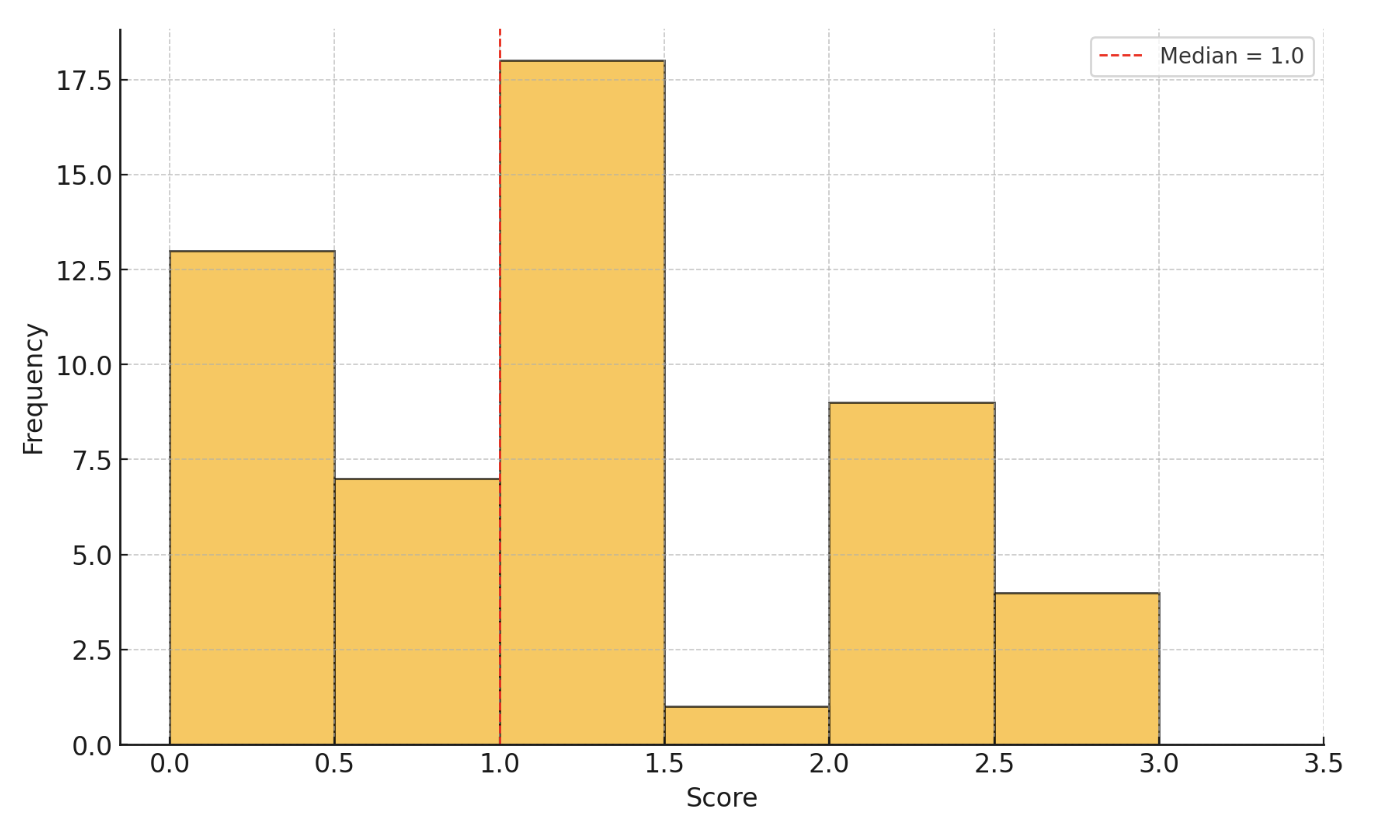
\includegraphics[width=.75\textwidth]{images/reading_quiz_scores_intro_to_relations}
   		 \caption{Median Extra Credit Score = 1/3}
\end{figure}
\vfill 
%\textbf{Remark.} Most people chose the set equality question. There were various issues with this that we will discuss in class today.  \alertstar Make sure you can answer the set equality question correctly for Friday's problems quiz \alertstar.
\end{frame}



\begin{frame}{Group Exercises: Introduction to Functions}

\begin{enumerate}
	\item Let $A=\set{1,2,3}$ and $B=\set{4,5}$.  Write down all functions $f: A \to B$. Indicate which are one-to-one and which are onto B.
	\item Let $A=\set{1,2}$ and $B=\set{3, 4,5}$.  Write down all functions $f: A \to B$. Indicate which are one-to-one and which are onto B.
	\item For each of the following relations, answer the following questions:
	(i) Is it a function? If not, explain why and stop. Otherwise, continue onward.
	(ii) What are its domain, codomain, and range?
	(iii) Is the function injective? 
	(iv) Is it surjective?
	\begin{itemize}
	\item[a)] $\set{(x,y): x,y \in \mathbb{Z}, y=2x}$
	\item[b)] $\set{(x,y): x,y \in \mathbb{Z}, xy=0}$
	\item[c)] $\set{(x,y): x,y \in \mathbb{Z}, y=x^2}$
	\end{itemize}
	\item Suppose $f: A \to B$ is a function where $A$ and $B$ are finite sets. Write psuedocode of an algorithm to test whether $f$ is bijective (a one-to-one correspondence).
	%\item (Bonus.) Prove that the composition of surjective functions is surjective. 
\end{enumerate}

\end{frame}


\begin{frame}{Solution to Group Exercise \#1}
\small 
\textbf{Problem.} Let $A=\set{1,2,3}$ and $B=\set{4,5}$.  Write down all functions $f: A \to B$. Indicate which are one-to-one and which are onto B.

\vfill 
\textbf{Solution.} There are 8 possible functions:
\begin{align*}
F_1 & \defeq \bigg\{ (1,4), (2,4), (3,4) \bigg\} & \quad F_5 & \defeq \bigg\{ (1,5), (2,4), (3,4) \bigg\} \\
F_2 & \defeq \bigg\{ (1,4), (2,4), (3,5) \bigg\} & \quad F_6 & \defeq \bigg\{ (1,5), (2,4), (3,5) \bigg\} \\
F_3 & \defeq \bigg\{ (1,4), (2,5), (3,4) \bigg\} & \quad F_7 & \defeq \bigg\{ (1,5), (2,5), (3,4) \bigg\} \\
F_4 & \defeq \bigg\{ (1,4), (2,5), (3,5) \bigg\} & \quad F_8 & \defeq \bigg\{ (1,5), (2,5), (3,5) \bigg\}
\end{align*}
%
Of these, all are onto except $F_1$ and $F_8$.   None of them are one-to-one.
\vfill
\textbf{Remark.} How did we know there were 8 possible functions? \pause   By the multiplication principle, there are $|B|^{|A|} = 2^3=8$ possible functions, because there are $|B|$ possible outputs for each of the $|A|$ inputs.   (When $A,B$ are finite, you can consider a function $A \to B$ as a \alert{list} with $|A|$ entries and $|B|$ choices for each entry.)
\end{frame}


\begin{frame}{Solution to Group Exercise \#2}
\small 
\textbf{Problem.}  Let $A=\set{1,2}$ and $B=\set{3, 4,5}$.  Write down all functions $f: A \to B$. Indicate which are one-to-one and which are onto B.
\vfill 
\textbf{Solution.} There are 9 possible functions:
\begin{align*}
F_1 & \defeq \bigg\{ (1,3), (2,3) \bigg\} & \quad F_4 & \defeq \bigg\{ (1,4), (2,3) \bigg\} & \quad F_7 & \defeq \bigg\{ (1,5), (2,3) \bigg\} \\
F_2 & \defeq \bigg\{ (1,3), (2,4) \bigg\} & \quad F_5 & \defeq \bigg\{ (1,4), (2,4) \bigg\} & \quad F_8 & \defeq \bigg\{ (1,5), (2,4) \bigg\} \\
F_3 & \defeq \bigg\{ (1,3), (2,5) \bigg\} & \quad F_6 & \defeq \bigg\{ (1,4), (2,5) \bigg\} & \quad F_9 & \defeq \bigg\{ (1,5), (2,5) \bigg\} \\
\end{align*}
%
Of these, none are onto.  All are one-to-one except $F_1$, $F_5$, and $F_9$.
\vfill
\textbf{Remark.} By the multiplication principle, we know there are $|B|^{|A|} = 3^2 = 9$ possible functions.
\end{frame}

\begin{frame}{Solution to Group Exercise \#3}
\footnotesize 
\textbf{Problem.} For each of the following relations, answer the following questions:
	(i) Is it a function? If not, explain why and stop. Otherwise, continue onward.
	(ii) What are its domain, codomain, and range?
	(iii) Is the function injective? 
	(iv) Is it surjective?
	\begin{itemize}
	\item[a)] $f_1 \defeq \set{(x,y): x,y \in \mathbb{Z}, y=2x}$
	\item[b)] $f_2 \defeq \set{(x,y): x,y \in \mathbb{Z}, xy=0}$
	\item[c)] $f_3 \defeq \set{(x,y): x,y \in \mathbb{Z}, y=x^2}$
	\end{itemize}
\vfill 
\textbf{Solution.}
\begin{itemize}
\item[(i)] Is it a function? $f_1$ and $f_3$ are functions because each $x$ maps to exactly one $y$.  $f_2$ is not a function because $x=0$ maps to more than one (in fact, infinitely many) $y$'s.
\item[(ii)] For all three functions, the domain and codomain are the integers. (This was explicitly stated in the problem.) The range for $f_1$ is the integers. The range for $f_3$ is the natural numbers (i.e., $\set{0,1,2,3,\hdots}$).  
\item[(iii)] $f_1$ is injective, but $f_2$ is not.  (Think: you can recover $x$ from $y$ for $f_1$, but not $f_2$).  
\item[(iv)] $f_1$ is surjective, but $f_2$ is not.  This is immediately clear from (ii), because a function is surjective if and only if its range equals its codomain. (Think: the realized function values covers the entire space of the codomain for $f_1$, but not $f_2$.)  
\end{itemize}


\end{frame}

\begin{frame}{Solution to Group Exercise \#4}
\footnotesize 
\textbf{Problem.} Suppose $f: A \to B$ is a function where $A$ and $B$ are finite sets. Write psuedocode of an algorithm to test whether $f$ is bijective (a one-to-one correspondence).
\vfill 

\begin{myredbox}[title=Psuedocode to test a function is bijective]
    \begin{algorithm}[H]
        %\SetAlgoLined
        \KwIn{A function $f: A \to B$, sets $A$ (domain), $B$ (codomain)}
        \KwOut{Determines if $f$ is bijective}
        \textbf{Initialize:} An empty set \texttt{seen\_values} \;
        \tcc{Check for injectivity}
         \For{each $x$ in $A$}{
            $y \gets f(x)$\;
            \If{$y$ is in \texttt{seen\_values}}{
                \textbf{Output:} "Not injective"\;
                \textbf{Exit}\;
            }
            Add $y$ to \texttt{seen\_values}\;
        }
        \tcc{Check for surjectivity}
        \eIf{\texttt{seen\_values} contains all elements of $B$}{
            \textbf{Output:} "Function is bijective"
        }{
            \textbf{Output:} "Not surjective"
        }
    \end{algorithm}
\end{myredbox}
\end{frame}


\end{document}
